
\documentclass[10pt]{article}

\usepackage{graphicx,amsmath,amssymb,subfigure,enumerate,versions}
\usepackage{multicol,multirow,mdframed}
\usepackage{epstopdf}
\usepackage{pstricks,auto-pst-pdf}
\usepackage{pst-all}
\usepackage{pst-ode}
\usepackage{pst-math}
\DeclareGraphicsExtensions{.png,.jpg,.pdf}

% ************ Page Margins *************
\hoffset=-1.3in
\setlength{\textwidth}{7.5in}
%%%%% MARGINS
\topmargin 0pt
\advance \topmargin by -\headheight
\advance \topmargin by -\headsep
\textheight 9.5in

% ************ Shortcuts *************
\newcommand{\Z}{\mbox{\sf Z\hspace{-1.5mm}Z}}
\newcommand{\SolutionSeparator}{ \hfill \hfill \hrule \hfill \hfill }
\newcommand{\R}{\mbox{\rm I\hspace{-0.75mm}R}}
\columnsep=0.75in
\newcommand{\vsc}{\vspace{1mm}}
\newcommand{\D}{\Delta }
\newcommand{\ifd}{f(x)~dx}
\newcommand{\dd}{\frac{dy}{dx} \,} 
\newcommand{\der}[2]{\frac{d{#1}}{d{#2}} \,}
\newcommand{\ddx}[1]{\frac{d {#1}}{dx} \,} 
\newcommand{\ddy}[1]{\frac{d {#1}}{dy} \,} 
\newcommand{\ddz}[1]{\frac{d {#1}}{dz} \,} 
\newcommand{\ddt}[1]{\frac{d {#1}}{dt} \,} 
\newcommand{\ds}{\displaystyle } 
\newcommand{\la}{\lambda } 
\newcommand{\del}{\nabla } 
\newcommand{\zx}{\frac{\partial z}{\partial x} \,}
\newcommand{\zy}{\frac{\partial z}{\partial y} \,}
\newcommand{\dx}{\frac{\partial f}{\partial x} \,}
\newcommand{\dy}{\frac{\partial f}{\partial y} \,}
\newcommand{\pp}[2]{\frac{\partial {#1}}{\partial {#2}} \,}
\newcommand{\ppx}{\frac{\partial }{\partial x} \,}
\newcommand{\ppy}{\frac{\partial }{\partial y} \,}
\renewcommand{\thesection}{\Roman{section}}
\newcommand{\vi}{\vec{i}}
\newcommand{\vj}{\vec{j}}
\newcommand{\vk}{\vec{k}}
\newcommand{\vv}{\vec{v}}
\newcommand{\lan}{\left\langle}
\newcommand{\ran}{\right\rangle}
\newcommand{\degr}{^{\circ}}

% *** Define the printed question style ***
\newcommand{\q}[1]{ {\em #1} }
% \renewcommand{\q}[1]{ {} }

\newcommand{\notice}{ \begin{center}Some problems and solutions
    selected or adapted from \\ Stewart {\em Calculus-Early
      Transcendentals} and Hughes-Hallett {\em Calculus} .\end{center}
}

% *** Overwrite, if desired, the question format
\input{DocumentFormat.tex}

% *** Footnoting with symbols ***
\long\def\symbolfootnote[#1]#2{\begingroup%
\def\thefootnote{\fnsymbol{footnote}}\footnote[#1]{#2}\endgroup}

\newcommand{\WeekTitleOne}{Derivatives - Foundations}
\newcommand{\WeekTitleTwo}{Derivatives - Linearization and Applications}
\newcommand{\WeekTitleThree}{Derivatives - Applications}
\newcommand{\WeekTitleFour}{Integrals - Foundations}
\newcommand{\WeekTitleFive}{Integrals - Techniques}
\newcommand{\WeekTitleSix}{Integrals - Modeling}
\newcommand{\WeekTitleSeven}{Differential Equations - }
\newcommand{\WeekTitleEight}{Differential Equations - }
\newcommand{\WeekTitleNine}{Differential Equations - }
\newcommand{\WeekTitleTen}{Linear Algebra - }
\newcommand{\WeekTitleEleven}{Linear Algebra - }
\newcommand{\WeekTitleTwelve}{Linear Algebra - }


\begin{document}


\begin{center}
\subsection*{MNTC P01 - Week \#3 - \WeekTitleThree}
\end{center}


\subsection*{Optimization Introduction}
\begin{enumerate}[1.]
\begin{multicols}{2}

\item
\begin{Question}
Let \(f(x)=x^{2}-10x+13\), and consider the interval \([0, 10]\). 
\begin{enumerate}[(a)]
\item  Find the critical point \(c\) of \(f(x)\) and compute \(f(c)\).
\item  Compute the value of \(f(x)\) at the endpoints of the interval \([0,10]\).
\item  Determine the global min and max of \(f(x)\) on \([0,10]\).
\item  Find the global min and max of \(f(x)\) on \([0,1]\). (Note: not the same interval as before)
\end{enumerate}
\par  \end{Question}
\begin{Solution}
  \begin{enumerate}[(a)]
  \item The critical point of \(f(x)\) is the solution to \(f'(x)=0\). The
  derivative is\(f'(x)=2x-10\). Setting this equal to zero and solving
  for \(x\) gives \(x=5\). Evaluating \(f(5)\) yields $-12$.
\item Evaluating \(f(0)\) and \(f(10)\), we find that each is equal to 13.
\item The global min and max values must occur at critical points or
  at the endpoints of the interval. Since the value at the critical
  point is smaller than the value at the endpoints, the value of
  \(f(5)\) is a minimum, and the value of \(f(0)\) (or \(f(10)\) since
  they are equal) is a maximum.
\item Since there are no critical points in the interval \([0,1]\), so
  the global min and max values lie at the endpoints of the
  interval. Computation yields \(f(0)=13\),\(f(1)=4\), so the minimum
  is 4 and the maximum is 13.
  \end{enumerate}
\par\end{Solution}
\item
\begin{Question}
Find the maximum and minimum values of the function \(\ds f(x)=\frac{\ln\!\left(x\right)}{x}\) on the interval [1,3]. 
\end{Question}
\begin{Solution}
  First we check for critical points. The critical point of \(f(x)\)
  is the solution to \(f'(x)=0\). \\
  The derivative
  is\(\ds f'(x)=x^{-2}-\frac{\ln\!\left(x\right)}{x^{2}}\). \\
  Setting this
  equal to zero and solving for \(x\) gives \(x=e^1=e\).\\
  Evaluating \(f(e)\) yields the value 
  \(\frac{1}{e}=0.3679\). \\
  The values of the function at the endpoints of the interval are
  \(f(1)=0\), \(f(3)=0.3662\), so the minimum value is 0, and the
  maximum value is \(\frac{1}{e}=0.3679\).
\par 
\par\end{Solution}
\item
\begin{Question}
  Find the minimum and maximum values of \(y = \sqrt{10}\theta-\sqrt{5}\sec\theta\) on the interval \([ 0, \frac {\pi}{3}]\).
\par  \end{Question}
\begin{Solution}
 
\par 
Let \(f(\theta) = \sqrt{10} \theta - \sqrt{5}\sec \theta\).  \leavevmode\\\relax 
On the interval \([ 0, \frac {\pi}{3}]\) , \(f'(\theta)= \sqrt{10} - \sqrt{5}\sec \theta \tan \theta = 0\)  at  \(\theta = \frac{\pi}{4}\).  \\
(This can be found either by inspiration, guessing that the answer is a `nice' angle like $\pi/3$, $\pi/4$ or $\pi/6$, or more mechanically by writing the whole equation in terms of $\sin(\theta)$, using $\cos^2(\theta) = 1 - \sin^2(\theta)$ and then solving a quadratic equation.) \\
The minimum value of  \(f\) on this interval is at \leavevmode\\\relax 
 the endpoint \(\theta=0\), where \(f(0) = -2.2361\), \leavevmode\\\relax 
whereas the maximum value over this interval is \leavevmode\\\relax 
\(f(\frac{\pi}{4})=\sqrt{10}(\frac{\pi}{4} - 1) = -0.6786\). \leavevmode\\\relax 
At the second endpoint \(\theta=\frac{\pi}{3}\), \leavevmode\\\relax 
 \(f(\frac{\pi}{3})= \sqrt{10} \frac{\pi}{3} - 2 \sqrt{5}= -1.1606\). 
\par\end{Solution}
\item
\begin{Question}
 
\par 
Find the maximum and minimum values of the function \(\ds f(x)=x-\frac{125x}{x+5}\) on the interval [0,21]. 
\par  \end{Question}
\begin{Solution}
 
First we check for critical points. The critical point of \(f(x)\) is
the solution to \(f'(x)=0\). \\
The derivative
is\(f'(x)=1-\frac{625}{\left(x+5\right)^{2}}\). \\
Setting this equal to
zero and solving for \(x\) gives \(x=-5\pm 25\), and of these two
critical points only -5+25=20 lies in our interval.\\
 Evaluating
\(f(-5+25)=f(20)\) yields the value -80.\\
 The values of the
function at the endpoints of the interval are \(f(0)=0\),
\(f(21)=-79.9615\), so the minimum value is -80, and the maximum value
is 0.
\par 
\par\end{Solution}
\item
\begin{Question}
 The function \(f(x) = -2 x^3 + 21 x^2 - 36 x + 10\)
has one local minimum and one local maximum. Find their $(x,y)$ locations.
\par\end{Question}
\begin{Solution}
  To identify any local extrema, we start by identifying critical
  points.  We note that $f(x)$ is a polynomial, so its derivative is
  defined everywhere, so only points where $f'(x) = 0$ will be
  critical points.
  \begin{align*}
    f'(x) & = -6x^2 + 42 x - 36 \\
\mbox{ Setting $f'(x) = 0$, }~~~~~~~ 0 & = -6 x^2 + 42 x - 36 \\
\mbox{ Factoring, }~~~~~~~ 0 & = -6 (x^2 - 7 x + 6) \\
0 & = -6 (x-1)(x-6) 
  \end{align*}
  The two critical points are at $x=1$ and $x=6$.  Subbing those $x$
  values back into the original function $f(x)$ gives us the points
  (1, -7) and $(6, 118)$.

Using test points and the first derivative test, or taking another derivative and using the second derivative test, you can find that:  \\
there is a local minimum at (1,-7), and \\
there is a local maximum at (6, 118).

\end{Solution}
\item
\begin{Question}
 A University of Rochester student decided to depart from Earth after his
graduation to find work on Mars.  Before building a shuttle, he conducted careful
calculations.  A model for the velocity of the shuttle, from liftoff at t = 0
s until the solid rocket boosters were jettisoned at t =   80 s, is given by
\[v(t) = 0.001094333 t^3- 0.08215 t^2 + 28.6 t - 4.3\] (in feet per
second).  Using this model, estimate the global
maximum value and global minimum value of the {\bf acceleration } of
the shuttle between liftoff and the jettisoning of the boosters.
\par\end{Question}
\begin{Solution}

For simplicity of presentation, let $c_3 =  0.001094333$ and $c_2 = 0.08215$, so
$$v(t) = c_3 t^3 - c_2 t^2 + 28.6 t - 4.3$$
Differentiating once gives the acceleration
$$a(t) = 3c_3 t^2 - 2c_2 t + 28.6 $$
To find the critical points of the acceleration, we need to know when its rate of change is
zero: 
$$a'(t) = 6 c_3 t - 2c_2 $$
This will have a zero value when 
\begin{align*}
  0 & = 6 c_3 t - 2c_2 \\
  t & = \frac{2c_2}{6 c_3} = \frac{1}{3} \frac{0.08215}{0.001094333} \approx 25.022
\end{align*}
Thus $t \approx 25.022$ is the only critical point.  

We compute the acceleration at the end points of the interval ($t=0$
and 80), and at the critical point: \\
$a(0)  = 28.6 \mbox{ ft/s}^2$ \\
$a(25.022)  = 26.5444 \mbox{ ft/s}^2$ \\
$a(80)  = 36.4672 \mbox{ ft/s}^2$ \\

The global maximum acceleration is $36.4672$ ft/s$^2$ and occurs at
$t=80$, while the global minimum acceleration is 26.5444 ft/s$^2$,
and it occurs at $t=25.022$ s.

\end{Solution}
\item
\begin{Question}
 Use the given graph of the function on the interval \((0,8]\) to answer the following questions.
\par 
\begin{center}
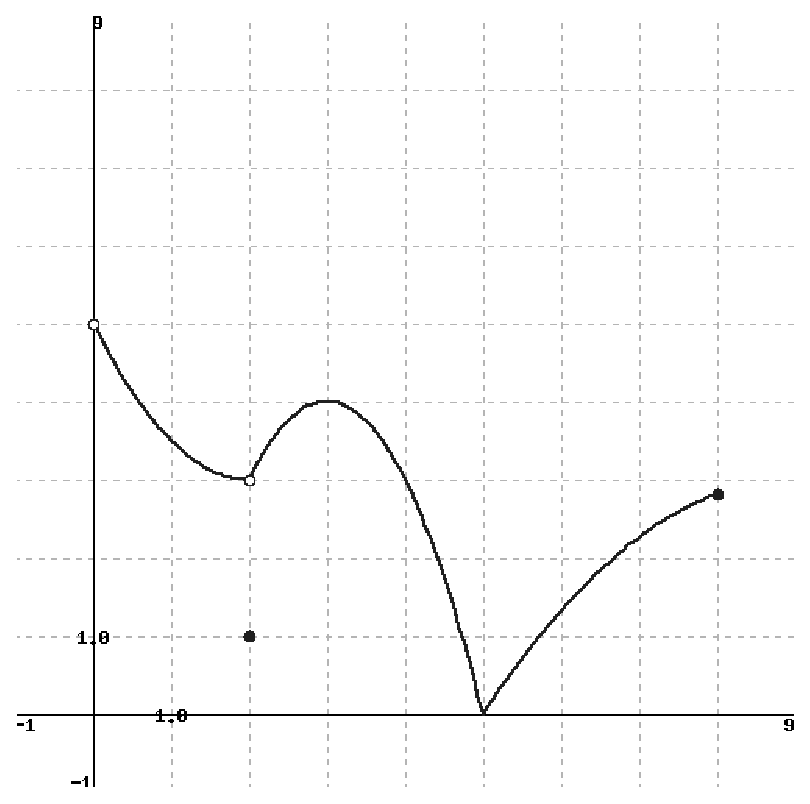
\includegraphics[width=0.7\linewidth]{graphics/Week03_OptimizationIntro/crit_point_graph}
\end{center} \par 
\begin{enumerate}[(a)]
\item Where does the function \(f\) have a local maximum?
\item Where does the function \(f\) have a local minimum?
\item What is the global maximum of \(f\)?
\item What is the global minimum of \(f\)?
\end{enumerate}
\par\end{Question}
\begin{Solution}
  \begin{enumerate}[(a)]
\item $x=$3.  ($x=8$ is an end-point, and so is {\bf not} considered a local max or min using our definitions.)
\item $x=$2, 5 
\item none:  at the left end, the interval is open, so the maximum is never reached.
\item The global minimum of the function occurs at $x=5$, and the value there is $f(5) = 0$.
  \end{enumerate}

\end{Solution}
\item
\begin{Question}
 \par 
Find the global maximum and minimum values of the following function on the given interval. 
\par 
\(f(t)= 4 t \sqrt{4-t^2}, \ [-1,2]\)
\par\end{Question}
\begin{Solution}  
The global maximum occurs at $x= 1.4142$ and $y = 8$. 

The global minimum occurs at $x=-1$, and $y = -6.9282$

\end{Solution}
\item
\begin{Question}
 \par 
 An object with weight W is dragged along a horizontal plane by a
 force acting along a rope attached to the object. If the rope makes
 an angle \(\theta\) with the plane, then the magnitude of the force
 is
\par 
$$F = \dfrac {\mu W} {\mu \sin ( \theta ) + \cos ( \theta ) }$$
\par 
where \(\mu\) is a positive constant called the coefficient of
friction and where \(0 \leq \theta \leq \pi/2\). Find the value for
\(\tan \theta\) which minimizes the force. Your answer may depend on W
and \(\mu\).
\par\end{Question}
\begin{Solution}
To minimize $F$, we differentiate with respect to $\theta$:
\begin{align*}
 &&   F(\theta) & = \mu W (\mu \sin(\theta) + \cos(\theta))^{-1} \\
\mbox{ so } &&  F'(\theta) & = - \frac{\mu W}{(\mu \sin(\theta) + \cos(\theta))^2}(\mu \cos(\theta) - \sin(\theta)) \\
\end{align*}
Setting the derivative equal to zero to identify critical points, 
\begin{align*}
0 & = - \frac{\mu W}{(\mu \sin(\theta) + \cos(\theta))^2}(\mu \cos(\theta) - \sin(\theta)) \\
\mbox{ requires } 0 & = (\mu \cos(\theta) - \sin(\theta)) \\
\sin(\theta) & = \mu \cos(\theta) \\
\frac{\sin(\theta)}{\cos(\theta)} & = \mu \\
\tan(\theta) & = \mu \\
\end{align*}
The question asked for the value of $\tan(\theta)$, so we have that now as $\mu$.

The greater the coefficient of friction, $\mu$, the more of our force
should be directed upwards rather than forwards, to help minimize the
friction effect.

\end{Solution}

\item
\begin{Question}
 Find the exact global maximum and minimum values of the
function \(f(t) = \frac{3 t}{8 + t^2}\) if its domain is all real
numbers.
\par  \end{Question}
\begin{Solution}
 
Differentiating using the quotient rule gives
\[f'(t)=\frac{3(8 + t^2) - 3 t(2 8 t)}{(8+t^2)^2} = 
    \frac{3(8 - t^2)}{(8+t^2)^2}.\]
The critical points are the solutions to
\(\frac{3(8 - t^2)}{(8+t^2)^2} = 0\), which are 
\(t = \pm\sqrt{8}\).
\par 
Since \(f'(t)>0\) for \(-\sqrt{8}<t<\sqrt{8}\) 
and \(f'(t)<0\) otherwise, there is a local
minimum at \(t=-\sqrt{8}\) and a local maximum at \(t=\sqrt{8}\). 
\par 
As \(t\to\pm\infty\), we have \(f(t)\to0\).  Thus, the local
maximum at \(t=\sqrt{8}\) is a global maximum of 
\(f(\sqrt{8}) = {3\sqrt{8}\over 8 + 8}\), 
and the local minimum at
\(t=-\sqrt{8}\) is a global minimum of 
\(f(-\sqrt{8}) = {-3\sqrt{8}\over 2(8)}\).
\par\end{Solution}
\item
\begin{Question}
 A ball is thrown up on the surface of a moon.  Its height
above the lunar surface (in feet) after \(t\) seconds is given by the formula
\[h=217 t-\frac{7}{4}t^2.\]
\begin{enumerate}[(a)]
\item Find the time that the ball reaches its maximum height.
\item Find the maximal height attained by the ball. 
\end{enumerate}
\par\end{Question}
\begin{Solution}
  \begin{enumerate}[(a)]
\item When the ball reaches its maximum, the velocity will be zero, so we can solve
for when velocity = $h'(t)$ = 0.

\begin{align*}
&& h'(t) & = 217 - \frac{7}{2} t \\
\mbox{ setting h'=0, } && 0 & = 217 - \frac{7}{2} t \\
&& t & = \frac{2}{7} 217 = 62 \mbox{ s}
\end{align*}
\item At the time of zero velocity, the height will be $h(62) = 6727$ m.
  \end{enumerate}
\end{Solution}
\item
\begin{Question}
 In a certain chemical reaction, substance \(A\) combines with substance 
\(B\) to form substance \(Y\).  At the start of the reaction, the
quantity of \(A\) present is \(a\) grams, and the quantity of 
\(B\) present is \(b\) grams.  Assume \(a<b\) and \(y\le a\).
At time \(t\)
seconds after the start of the reaction, the quantity of \(Y\)
present is \(y\) grams.  For certain types of reactions, the rate of
the reaction, in grams/sec, is given by 
\[\hbox{Rate}=k(a-y)(b-y),\]
where \(k\) is a positive constant.
\begin{enumerate}[(a)]
\item Sketch a graph of the rate against \(y\).
\item For what values of \(y\) is the rate non-negative?
\item Use your graph to find the value of \(y\) at which the rate of the 
reaction is fastest.
\end{enumerate}

\par  \end{Question}
\begin{Solution}

  \begin{enumerate}
\item~ \\ 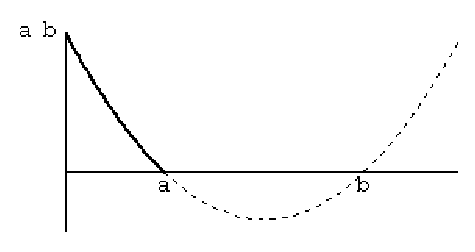
\includegraphics[width=0.75\linewidth]{graphics/Week03_OptimizationIntro/parabola_ab}
\par 
 
\item If we expect the rate to be non-negative, we must have \(0\le y\le a\)
or \(b \le y\).  Since we assume \(a<b\), we restrict \(y\) to 
\(0\le y\le a\).

In fact, the expression for the rate is non-negative for \(y\) greater
than $a$ but these values of \(y\) are not meaningful for the
reaction.  See the figure above (which shows the rate with \(k=1\)).
\par 
\item From the graph, we see that the maximum rate occurs when \(y=0\); that
is, at the start of the reaction.
  \end{enumerate}
\par\end{Solution}
\item
\begin{Question}
  At what value(s) of \(x\) on the curve \(y = 1 + 250 x^3 - 3 x^5\)
  does the tangent line have the largest slope?
\par\end{Question}
\begin{Solution}
The slope of the tangent line is given by $y' = 750 x^2 -15 x^4$.

Consider this to be a new function, $g(x)$, that we want to maximize (to get the {\em largest} slope).  To maximize $g(x)$, we differentiate to find critical points:
\begin{align*}
  g(x) & = 750 x^2 -15 x^4 \\
\mbox{ so } g'(x) & = 1500 x - 60 x^3 \\
\mbox{ set $g'$ = 0: } 0 & = 1500 x - 60 x^3 \\ 
0 &= 60x (25 - x^2) \\
0 &= 60x (5 - x)(5+x) \\
x & = 0, 5, -5
\end{align*}
These are the critical points of the slope function.  To determine
which is a max, and which is a min, we can use either the first or second derivative tests.
Let's use the 2nd here because differentiation of $g'$ will be easy:
$g''(x) = 1500  - 180 x^2$ \\
$g''(-5) = -3000 < 0$: concave down; $x=-5$ is a local max. \\
$g''(0) = 1500 > 0$: concave up; $x=0$ is a local min. \\
$g''(5) = -3000 < 0$: concave down; $x=5$ is a local max. \\

The values of $g(-5) = 9375$ and $g(5) = 9375$ are the slopes of the
original function at $x=-5$ and $x=5$.  They are equal, so they are
both the common global maximum slope of $9375$.
\end{Solution}

\end{multicols}
\hrulefill

\begin{multicols}{2}

\subsection*{Optimization With MATLAB}

For Questions \ref{qoptmatlab1}-\ref{qoptmatlab2}, use MATLAB to:
\begin{itemize}
\item generate a graph of the given function on the domain shown, and
\item use the \texttt{fminbnd} function to find the global maximum and
  global minimum of the function on that interval.
\end{itemize}

% ******************************
\item \label{qoptmatlab1}
\begin{Question}
$f(x)= 7 e^{7 x^3 -  7 x} , \mbox{ on }  -1 \leq x \leq 0$
\end{Question}
\begin{Solution}

All the examples will be solved with the same basic architecture. 

In the MATLAB plots, 
\begin{itemize}
\item the global {\bf min} will be shown as a {\bf red} dot, and
\item the global {\bf max} will be shown as a {\bf green} dot.
\end{itemize}

If there is anything special that is required in the solving, it will
be mentioned in text, as well as a commetn in the MATLAB code.

\href{http://www.mast.queensu.ca/~apsc171/MNTCP01/PracticeProblems/MATLAB/W03OptExp1.m}{W03OptExp1.m}

\lstinputlisting{MATLAB/W03OptExp1.m}

Final answer:
\begin{verbatim}
Global min (x, y) 
   -0.0001    7.0032

Global max (x, y) 
   -0.5774  103.5662
\end{verbatim}

\end{Solution}
% ******************************
\item
\begin{Question}
$f(x)= 7 x - 21 \ln (x),\mbox{ on } \ [1,4]$
\par\end{Question}
\begin{Solution}

  For all the following problems, we will just provide a link to the
  solution MATLAB file, and the final answer, rather than including it
  in the PDF.

  Looking at the graph, this function has a clear global max at the
  left boundary of the interval, and a global min at the critical
  point at $x=1$.

\href{http://www.mast.queensu.ca/~apsc171/MNTCP01/PracticeProblems/MATLAB/W03OptLn1.m}{W03OptLn1.m}

\begin{verbatim}
Global min (x, y) 
    3.0000   -2.0709

Global max (x, y) 
    1.0000    6.9994
\end{verbatim}

\end{Solution}
% ******************************
\item
\begin{Question}
 \par 
$f(x)= 4 e^{-x} - 4 e^{-2 x}, \mbox{ on }\ [0,1]$
\end{Question}
\begin{Solution}
  Looking at the graph, this function has a clear global max at the
  left boundary of the interval, and a global min at the critical
  point at $x\approx 0.6931$ (exact value is $x = \ln(2)$).

\href{http://www.mast.queensu.ca/~apsc171/MNTCP01/PracticeProblems/MATLAB/W03OptExp2.m}{W03OptExp2.m}

Notice that MATLAB doesn't return {\em exactly} $x=0$ for the global
minimum, but just the very small
$x = 0.0661\times 10^{-3} = 0.0000661$.  This kind of slight deviation
from the exact value is common with numerical methods.

\begin{verbatim}
Global min (x, y) 
   1.0e-03 *

    0.0661    0.2644

Global max (x, y) 
    0.6931    1.0000
\end{verbatim}

\end{Solution}
% ******************************
\item
\begin{Question}
$f(x)= 7 x - 14 \cos (x), \mbox{ on }  [-\pi,\pi]$
\par\end{Question}
\begin{Solution}
  Looking at the graph, this function has 
  \begin{itemize}
  \item a clear global max at the
  right boundary of the interval, and 
\item a global min at the critical point at $x\approx -0.5236$.
  \end{itemize}

  There is a local max around $x=-2.8$ that isn't found by
  \texttt{fminbnd} when the interval is $[-\pi, pi]$.

\href{http://www.mast.queensu.ca/~apsc171/MNTCP01/PracticeProblems/MATLAB/W03OptTrig1.m}{W03OptTrig1.m}

\begin{verbatim}
Global min (x, y) 
   -0.5236  -15.7895

Global max (x, y) 
    3.1415   35.9907
\end{verbatim}


\end{Solution}
% ******************************
\item
\begin{Question}
 \par 
$f(x)= ( 3 \cos x ) / (20 + 10 \sin x ), \ 0 \leq x \leq 2 \pi$
\par\end{Question}
\begin{Solution}

  This example requires some care, as the default search with
  \texttt{fminbnd} does {\bf not} find the correct global maximum.

\href{http://www.mast.queensu.ca/~apsc171/MNTCP01/PracticeProblems/MATLAB/W03OptTrig2.m}{W03OptTrig2.m}

\begin{verbatim}
Global min (x, y) 
    3.6652   -0.1732

Endpoint (x, y) 
    0.0001    0.1500

Global max (x, y) 
    5.7596    0.1732
\end{verbatim}
\end{Solution}
% ******************************
\item\label{qoptmatlab2}
\begin{Question}
 \par 
 \(f(t)=\frac{10}{t}+4, 0 < t \leq 1\)  \\
 Note the open end due to the $0 < t$ instead of $0 \le t$.
\par\end{Question}
\begin{Solution}

  {\bf Variables}: note that you can choose to change the $x$
  variables in your script to \texttt{t}, or just note that the
  function $\ds f(x) = \frac{10}{x} + 4$ has all the same properties
  as $\ds f(t) = \frac{10}{t} + 4$.

  {\bf Open Interval: }Even though we are working on an open interval,
  we can still try to use \texttt{fminbnd}.  We just need to be
  careful when running it, and interpreting its results.

\href{http://www.mast.queensu.ca/~apsc171/MNTCP01/PracticeProblems/MATLAB/W03OptRecip1.m}{W03OptRecip1.m}

  If you run your \texttt{fminbnd} with $t=0$ as a boundary, you will get an error:
\begin{verbatim}
Error using fminbnd (line 219)
User supplied objective function must return a scalar value.
\end{verbatim}
  This points to the fact that $f(0)$ is actually undefined (dividing
  by zero).  As a result, the best you can do is try to use a small
  but non-zero left limit, but then check your results against the
  graph to be sure.

\begin{verbatim}
Global min (x, y) 
    0.9999   14.0005

Global max (x, y) 
   1.0e+04 *

    0.0000    6.0209
\end{verbatim}
  {\bf However}, the global max is actually incorrect.  This function won't have a global max, 
  because there is a vertical asymptote at $t=0$, so there is no single highest point for this function.

\end{Solution}

\end{multicols}
\hrulefill
\subsection*{Optimization Word Problems}

\begin{multicols}{2}

% ******************************
\item
\begin{Question}
 Some airlines have restrictions on the size of items of luggage that
passengers are allowed to take with them.  Suppose that one has a rule
that the sum of the length, width and height of any piece of luggage
must be less than or equal to 192 cm.  A passenger wants to take a
box of the maximum allowable volume.    
\begin{enumerate}[(a)]
\item If the length and width are to
be equal, what should the dimensions be?
\item In this case, what is the volume? 
\item If the length is be twice the width, what should the dimensions be? 
\item In this case, what is the volume? 
\end{enumerate}
Include units in all your answers.
\par  \end{Question}
\begin{Solution}
 
  Let the length, width and height of the box be \(L\), \(w\) and
  \(h\), respectively.  Then the volume of the box is \(V = Lwh\).
  The sum \(L + w + h = 192\), and, for the first part, we know that
  \(L = w\).  Thus \(2w + h = 192\), so \(h = 192 - 2w\), and the
  volume equation becomes \(V = Lwh = w\cdot w\cdot(192 - 2w) =
  192\cdot w^2 - 2w^3\).  Since we need $h \ge 0$ and $h = 192 - 2w$,
  the domain for \(w\) is \(0\le w\le 96\).
\par 
Critical points are where 
\(\frac{dV}{dw} = 2\cdot 192\cdot w - 6\cdot w^2 = 0\), so 
\(w = 0\) or \(w = 64\).  The global maximum must occur either at
this point or at the end points.  \(V(64) > 0\) while 
\(V(0) = V(96) = 0\), so the global maximum is at \(L=w=64\), 
in which case \(h=64\) as well.  The volume is then 
\(V = 64^3 = 262144 {\rm cm}^3\).
\par 
If \(L = 2w\), \(2w + w + h = 192\), so 
\(V = (2w)(w)(192 - 3w) = 384 w^2 - 6 w^3\).  Proceeding as
before, we find \(w = \frac{128}{3}\), \(L = \frac{256}{3}\) and \(h = 64\), so that 
\(V = \frac{2097152}{9}\).
\par\end{Solution}
% ******************************
\item
\begin{Question}
 A wire 3 meters long is cut into two pieces.  One piece is bent
into a square for a frame for a stained glass ornament, while the
other piece is bent into a circle for a TV antenna.  
\begin{enumerate}[(a)]
\item To reduce storage
space, where should the wire be cut to {\bf minimize} the total area of both
figures? 
\item Where should the wire be cut to {\bf maximize} the total area?  
\end{enumerate}
\par  \end{Question}
\begin{Solution}
  \begin{enumerate}[(a)]
  \item Note that we are interested in {\it the total area enclosed by
the two figures} .  Our first task is therefore to find an
equation for this area, which will be the sum of the areas of the two
figures.
\par 
Suppose we cut \(x\) meters of wire to make the circular antenna.
Then there are \(3 - x\) meters left for the square.  To find the
area of the circle we need its radius.  The circumference of a circle
of radius \(r\) is \(C = 2\pi r\), so the radius of the circle is
given by \(2\pi r = x\), and so \(r = \frac{x}{2\pi}\).  The area
of the circular antenna is therefore 
\(A_c = \pi r^2 = \frac{1}{4\pi} x^2\).
\par 
Then the perimeter of a square with side length \(s\) is 
\(P = 4 s = 3 - x\), so the side length is 
\(s = \frac{1}{4}(3 - x)\).  Then the area of a square is 
\(A_s =  s^2\), so the area of the square is 
\(A_s =  (\frac{1}{16})(3 - x)^2\).
\par 
The total area is therefore
\[A = \frac{1}{4\pi} x^2 +  (\frac{1}{16})(3 - x)^2
  = \frac{1}{4\pi} x^2 + \frac{1}{ (16)}(9 - 6 x + x^2).\]
The domain for \(x\) is \(0\le x\le 3\).  
\par  
The maximum and minimum of \(A\) will occur at critical or end
points.  Critical points are where \(dA/dx = 0\), or, where
\[\frac{1}{2\pi} x + \frac{1}{ (16)}(2x - 6) = 0.\]
Collecting all terms in \(x\) we have
\[\left( \frac{1}{2\pi} + \frac{2 }{ (16)}\right) x = 
  \frac{6 }{16},\]
so, after simplifying, 
\[x = \frac{3 \pi}{4 + \pi}.\]
\par 
To determine if this is a local maximum or minimum, we use the second
derivative test.  
\[A'' = \left( \frac{1}{2\pi} + \frac{2 }{ (16)}\right) > 0,\]
so the function is concave up everywhere and this is a local minimum.
Also, because this is the {\em only} critical point, this is also a {\em global}
minimum for the area.

Thus to minimize area we use \(\frac{3 \pi}{4 + \pi}\) meters of wire
for the circle and \(3 - \frac{3 \pi}{4 + \pi}\) meters for the
square.
\item To {\em maximize} the area, we can't use our critical point,
  which was a minimum; instead we must use the endpoints.  The areas
  at the endpoints are
\[A(0) = \frac{9}{16} \approx 0.56\qquad{\rm and}\qquad
   A(3) = \frac{9}{4\pi} \approx 0.72,\]
the larger of which is \(A(3)\), so the maximum area occurs when
all of the wire is used for the circle and none for the square.
  \end{enumerate}
\par\end{Solution}
% ******************************
\item
\begin{Question}
 A printed poster is to have a total area of 799 square inches with top and
bottom margins of 6 inches and side margins of 4 inches. What should be the
dimensions of the poster so that the printed area be as large as possible?
Let \(x\) denote the width of the poster and let \(y\)
denote the length. 

\includegraphics[width=0.7\linewidth]{graphics/Week03_OptimizationWordProblems/Poster}

\begin{enumerate}[(a)]
\item Write the function of $x$ and $y$ that you need to maximize.
\item Express that function in terms of $x$ alone. 
\item Find the critical points of the function. 
\item Use the second derivative test to verify that \(f(x)\) has a maximum at this critical point 
\item Find the optimal dimensions of the poster, and the resulting area.  Include units.
\end{enumerate}
\par\end{Question}
\begin{Solution}
  \begin{enumerate}[(a)]

\item $\mbox{Area} = A = (x-2\cdot 4 )(y - 2\cdot 6)= (x - 8)(y - 12)$
\item By using the requirement that $799 = x y$, we get  $A = (x - 8)(799/x - 12)$
\item Differentiating and setting the derivative equal to zero, we obtain $x = 23.08$.
\item The second derivative of $A$ will be negative at $x = 23.08$, so
  $A$ is concave down there, indicating $x=23.08$ is a local maximum for the printed area.
\item The dimensions of the poster with the largest printed area will be
$23.08 \times 34.62$, with a net printed area of 341.09 cm.
  \end{enumerate}

\end{Solution}
% ******************************
\item
\begin{Question}
 A box with an open top has vertical sides, a square bottom, and a volume of
32 cubic meters. If the box has the least possible surface area, find its
dimensions.
\par\end{Question}
\begin{Solution}
This is the same question studied in the course videos.  Let the dimensions
of the box be $w$ and $h$; the bottom is square so $w$ can represent the length of both 
sides of the bottom.  These combine to produce
$$A = w^2 + 2(wh) + 2(wh), ~~~~ V = w^2h = 32$$
Solving for $h$ in the $V$ equation, $\ds h = 32/w^2$, we can write
$A$ as just a function of $w$:
\begin{align*}
A & = w^2 + 4w(32/w^2) \\
A & = w^2 + 128/w \\
\end{align*}
Differentiating and setting $A' = 0$, you will find $w = 4$, and consequently $h = 32/w^2 = 2$.

\end{Solution}
% ******************************
\item
\begin{Question}
 Find the dimensions of the rectangle of largest area that can be
inscribed in an equilateral triangle with sides of length 2 if 
one side of the rectangle lies on the base of the triangle.
\par\end{Question}
\begin{Solution}
The optimal rectangle will be 1 unit on the base, and have height $\ds \frac{\sqrt{3}}{2}$.

\end{Solution}
% ******************************
\item
\begin{Question}
 Find the minimum distance from the parabola 
 \[x - y^2 = 0\]  to the point {(0,3)}.
\par\end{Question}
\begin{Solution}


The point of closest approach will occur at $y=1$, and that will give a distance
of $\sqrt{ 1^2 + (3-1)^2} = \sqrt{5}$.
\end{Solution}
% ******************************
\item
\begin{Question}
  I have enough pure silver to coat \(2\) square meters of surface
  area.  I plan to coat a sphere and a cube.
  \begin{enumerate}[(a)]
  \item Allowing for the possibility of all the silver going onto one
    of the solids, what dimensions should they be if the total volume
    of the silvered solids is to be a maximum? 
  \item Now allowing for the possibility of all the silver going onto
    one of the solids, what dimensions should they be if the total
    volume of the silvered solids is to be a minimum? 
  \end{enumerate}
\par  \end{Question}
\begin{Solution}
 
  Let \(s\) be the length of the cube, \(A\) the total area, and \(V\)
  the total volume.  Then
\[A=4\pi r^2+6s^2\]
and
\[V= \frac{4}{3}\pi r^3 + s^3.\]
Obviously, the volume is maximized if we put all of our stock in the
sphere.  In that case, 
\[r = \sqrt{\frac{A}{4\pi}} \approx 0.3989\hbox{~meters}\]
(and \(s=0\) meters).
To minimize the volume we eliminate one of the variables and find a
stationary point as usual.
Solving the area equation for \(s\) gives
\[s= \sqrt{\frac{A-4\pi r^2}{6}}.\] Substituting this value in the
volume equation gives
\[V= \frac{4}{3}\pi r^3 + \left(\frac{A-4 \pi
r^2}{6}\right)^{\frac{3}{2}}.\]
Differentiating with respect to \(r\) and setting to zero gives:
\[V'=4\pi r^2 - \frac{3}{2}\times\frac{8\pi r}{6} \left(\frac{A-4 \pi
r^2}{6}\right)^{\frac{1}{2}} = 0.\]
This simplifies to
\[2r = \sqrt{\frac{A-4 \pi
r^2}{6}}.\]
Squaring gives
\[4r^2 = \frac{A-4 \pi
r^2}{6}\]
which gives
\[r = \sqrt{\frac{A}{24+4\pi}} \approx  0.2339\hbox{~meters.}\]
The corresponding value of \(s\) is
\[s = 2r = \sqrt{\frac{A}{6+\pi}} \approx  0.4677\hbox{~meters.}\]
\par\end{Solution}
% ******************************
\item
\begin{Question}
Suppose that 241 ft of fencing are used to enclose a corral in the shape of a rectangle with a semicircle whose diameter is a side of the rectangle as the following figure:\leavevmode\\\relax 
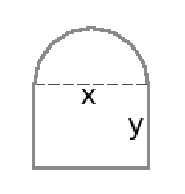
\includegraphics[width=0.3\linewidth]{graphics/Week03_OptimizationWordProblems/WindowShape}

Find the dimensions of the corral with maximum area. 
\par  \end{Question}
\begin{Solution}
 
\par 
From the picture, we see that \(x\) is the width of the corral, and therefore the diameter of the semicircle, \leavevmode\\\relax  and that \(y\) is the height of the rectangular section. Thus the perimeter of the corral can be expressed \leavevmode\\\relax 
by the equation \(2y+ x+ \frac{\pi}{2}x= 2y + (1+ \frac{\pi}{2})x= 241\) ft or equivalently, \leavevmode\\\relax 
\(y=\frac{1}{2}(241 - (1+ \frac{\pi}{2})x)\). Since \(x\) and \(y\) must both be non-negative, it follows that \(x\) must \leavevmode\\\relax 
be restricted to the interval \([0, \frac{241}{1+ \pi/2}]\). The area of the corral is the sum of the area of the \leavevmode\\\relax 
rectangle and semicircle, \(A= xy + \frac{\pi}{8}x^2\). Making the substitution for \(y\) from the \leavevmode\\\relax 
constraint equation, \par 
\(A(x)=\frac{1}{2}x(241 - (1+ \frac{\pi}{2})x) + \frac{\pi}{8}x^2 = 120.5 x - \frac{1}{2}(1+ \frac{\pi}{2})x^2 + \frac{\pi}{8}x^2\). \leavevmode\\\relax 
Now, \(A'(x) = 120.5 - (1 + \frac{\pi}{2})x + \frac{\pi}{4}x = 0\) implies \(x= \frac{120.5}{(1+ \frac{\pi}{4})} \approx 67.4919\).  \leavevmode\\\relax 
With \(A(0)=0\), \par 
\(A(\frac{120.5}{(1+ \frac{\pi}{4})}) \approx 4066.39 \qquad\) and \(\qquad A(\frac{241}{1+ \frac{\pi}{2}}) \approx 3451.11\), \leavevmode\\\relax 
it follows that the corral of maximum area has dimensions \par 
\(x= \frac{120.5}{1+ \frac{\pi}{4}} \qquad\) and \\
\(\qquad y= \frac{1}{2}(241 - (1+ \frac{\pi}{2}) \frac{120.5}{1+ \frac{\pi}{4}}) \approx 33.746\).
\par\end{Solution}
% \item
% \begin{Question}
 
% \par 
% Find the maximum area of a triangle formed in the first quadrant by the \(x\)-axis, \(y\)-axis and a tangent line to the graph of \(f=(x + 2)^{-2}\).
% \par  \end{Question}
% \begin{Solution}
 
% Let \(P\left(t,\frac{1}{(t+2)^2}\right)\) be a point on the graph of the curve \(y=\frac{1}{(x+2)^2}\) in the first quadrant. The tangent line to the curve at \(P\) is
% \[L(x)=\frac{1}{(t+2)^2}-\frac{2(x-t)}{(t+2)^3},\]
% which has \(x\)-intercept \(a=\frac{3t+2}{2}\) and \(y\)-intercept \(b=\frac{3t+2}{(t+2)^3}\). The area of the triangle in question is
% \[A(t) = \frac{1}{2}ab = \frac{(3t+2)^2}{4(t+2)^3}.\]
% Solve
% \[A'(t) = \frac{(3t+2)(3\cdot 2-3t)}{4(t+2)^4} = 0\]
% for \(0 \le t\) to obtain \(t = 2\).  Because \(A(0) = \frac{1}{4 \cdot 2}\), \(A(2) = \frac{1}{2 \cdot 2}\) and \(A(t) \to 0\) as \(t \to \infty\), it follows that the maximum area is \(A(2) = 0.25\).
% \par\end{Solution}
\item
\begin{Question}
 
\par 
A box is constructed out of two different types of metal. The metal for
the top and bottom, which are both square, costs \$4 per square foot
and the metal for the sides costs \$6 per square foot. Find the
dimensions that minimize cost if the box has a volume of 35 cubic
feet.
\par  \end{Question}
\begin{Solution}
 
Let \(x>0\) be the length of a side of the square base and \(z>0\) the height of the box. With volume \(x^{2} z=35\), we have \(z=35/x^{2}\) and cost
\[C(x)=4\cdot 2\cdot x^{2}+6\cdot 4\cdot xz=8x^{2}+840\frac{1}{x}.\]
Solve \(C'(x)=8\cdot 2x-840x^{-2}=0\) to obtain \(x= \left(\frac{35 \cdot 6}{4} \right)^{1/3}\). 
Since \(C(x) \to \infty\) as \(x \to 0+\) and as \(x \to \infty\), the minimum cost is 
\(C\left( (\frac{35 \cdot 6}{4})^{1/3} \right)
\approx \$ 336.499\) 
when 
\(x\approx 3.74444\textrm{ ft}\) 
and 
\(z\approx 2.49629\textrm{ ft}\).
\par\end{Solution}
%\item
%\begin{Question}
% A manufacturer has been selling 1550 television sets a week at \$540
% each.  A market survey indicates that for each \$23 rebate offered to
% a buyer, the number of sets sold will increase by 230 per week.  
% \begin{enumerate}[(a)]
% \item Find the price, $p(x)$, as a function of $x$, where \(x\) is
%   the number of the television sets sold per week.
% \item How large rebate should the company offer to a buyer, in order
%   to maximize its revenue?
% \item If the weekly cost function is \(139500 + 180 x\), how should
%   it set the size of the rebate to maximize its profit?
% \end{enumerate}
%\par\end{Question}
%\begin{Solution}
% \begin{enumerate}[(a)]
%\item $p(x) = (1550-x)/10 +540$.
%\item Revenue = price $\times$ demand = $(540 - 23\cdot x) (1550-x)/10 +540$.
%Finding the critical point of the revenue function, you will find $x = 192.5$.
%\item Build profit as revenue - cost. Compute the critical points, and
% you will find $x= 102.5$ produces a maximum profit.
% \end{enumerate}
%
%\end{Solution}
% \item
% \begin{Question}
%   A baseball team plays in he stadium that holds 72000
%   spectators. With the ticket price at 12 the average attendence has
%   been 30000. When the price dropped to 11, the averege attendence
%   rose to 36000.  \leavevmode\\\relax 
%   \begin{enumerate}[(a)]
%   \item Find the demand function \(p(x)\), where \(x\) is the number
%     of the spectators. (assume \(p(x)\) is linear.)
%   \item How should be set a ticket price to maximize revenue?
%   \end{enumerate}
% \par\end{Question}
% \begin{Solution}
%  {
% \vspace{-\parskip}\begin{itemize}
% \item $(30000-x)*1/(6*1000) +12$
% \item 8.5 
% \end{itemize}}\par
%\end{Solution}
%\item
%\begin{Question}
% For the cost function \(C(x) = 40000+800 x + x^2\) find: 
% \begin{enumerate}[(a)]
%\item The cost at the production level 1650.
%\item The average cost at the production level 1650.
%\item The marginal cost at the production level 1650 (this is the in.
%\item The production level that will minimize the average cost.
%\item The minimal average cost.  
% \end{enumerate}
%\par\end{Question}
%\begin{Solution}
%  \begin{enumerate}[(a)]
%\item 4082500 
%\item 2474.24242424242 
%\item 4100 
%\item 200 
%\item 1200 
%  \end{enumerate}
%
%\end{Solution}
% \item
% \begin{Question}
%   A rectangle is inscribed with its base on the \(x\) axis and its
%   upper corners on the parabola \(y= 12 - x^2\).  What are the
%   dimensions of such a rectangle with the greatest possible area?
% \par  \end{Question}
% \begin{Solution}
 
% To solve this problem, we need to find an expression for the area of the 
% rectangle in terms of one of its dimensions, and then use derivatives to
% maximize this area.  First, however, we can simply things quite a bit by 
% noting that the parabola given by \(y = 12 - x^2\) is symmetric about 
% the \(y\)-axis.  Therefore, the inscribed rectangle will also be symmetric 
% about the \(y\)-axis.  So it is enough to find the dimensions of half of this 
% rectangle and double the x value.
% \par 
% Our rectangle will therefore have the bottom left corner \((0,0)\) and the top
% right corner \((x,12-x^2)\) where \(x\) is the width of the rectangle, 
% and \(12 - x^2\) is its height.  Thus, the area of the rectangle is
% given by \(f(x) = x(12-x^2) = {12}x-x^3\) where \(x\) is the width 
% of the rectangle.  We now find the derivative of this and solve for zero 
% to find critical points.
% \par 
% The derivative is \(f'(x) = 12 - 3x^2\).  Setting this equal to 0 and 
% recalling that we are talking about widths, so that all \(x\) values 
% should be positive, we get:
% \par 
% \[\begin{aligned}
%     f'(x) & = 0 \\
%     12 - 3x^2 & = 0 \\
%     3x^2 & = 12 \\
%      x^2 & = \frac{12}{3} = 4 \\
%      x & = \sqrt{4} = 2
%   \end{aligned}\]
% \par 
% It is easy to check that the second derivative of \(f(x)\) is negative everywhere, 
% so this is a maximum of \(f(x)\).  Therefore, this is the width of the rectangle with the
% maximum area. Actually, it is the width of half of that rectangle, since we were
% ignoring the half on the left side of the y-axis. So the width of the whole rectangle is \(2\cdot 2 =  4\).  The height is given by 
% plugging \(x=2\) into the formula for the parabola, giving
% \(12 - (2)^2  = 12 - 4 = 8 \).
% \par\end{Solution}
\item
\begin{Question}
 Centerville is the headquarters of Greedy Cablevision Inc. The
cable company is about to expand service to two nearby towns,
Springfield and Shelbyville.  There needs to be cable connecting
Centerville to both towns.  The idea is to save on the cost of
cable by arranging the cable in a Y-shaped configuration.
Centerville is located at
\((8,0)\) in the \(xy\)-plane, Springfield is at \((0,5)\), and
Shelbyville is at \((0,- 5)\). The cable runs from Centerville
to some point \((x,0)\) on the \(x\)-axis where it splits into two branches going to
Springfield and Shelbyville. Find the location \((x,0)\)
that will minimize the amount of cable between the 3 towns and
compute the amount of cable needed. Justify your answer.
\par 
\begin{enumerate}[(a)]
\item What function of $x$ needs to be minimized to solve this problem?
\item Find the critical points of $f(x)$.
\item Use the second derivative test to verify that \(f(x)\) has a minimum at this critical point.
\item Compute the minimum amount of wire needed.
\end{enumerate}
\par\end{Question}
\begin{Solution}
  \begin{enumerate}[(a)]
\item Draw a sketch.   \\
\includegraphics[width=0.7\linewidth]{graphics/Week03_OptimizationWordProblems/Cablevision}

With $x$ being the horizontal component of the diagonal lines, the
total length of the cable will be $L(x) = 2 \sqrt{x^2+5^2}+(8 -x)$.
\item Taking the derivative and finding critical points of $L(x)$ yields $x = 2.89$.
\item The second derivative of $L(x)$ will be positive at $x = 2.89$, indicating that
the critical point is a local minimum for the length of cable. 
\item $L(2.89) = 2 \sqrt{(2.89)^2 + 25} + (8-2.89) = 16.66$ units of cable.
  \end{enumerate}

\end{Solution}
\item
\begin{Question}
  A cylinder is inscribed in a right circular cone of height 4 m and
  radius (at the base) equal to 3.5 m.  What are the dimensions of
  such a cylinder which has maximum volume?
\par  \end{Question}
\begin{Solution}
 
As we are attempting to maximize the volume of the inscribed cylinder,
we must first come up with a formula for the volume of this cylinder.
Let \(x\) be the radius of the cylinder, \(v(x)\) the volume.  We 
know from basic geometry that the formula for volume is give by 
\(\pi x^2h\) where \(x\) is the radius and \(h\) is the height
of the cylinder.  So in order to come up with a formula for volume
in terms of \(x\) only, we need to relate \(x\) to \(h\).
\par 
This is where the information about the cone comes in handy.  The cone is 
a right circular cone.  Thus, inscribing the cylinder will fill up
some of the base of the cone, and just touch the slanted side, leaving
a similar right circular cone at the top.  This new cone will have a
radius of \(x\) and a height of \(4 - h\) where \(x\) and \(h\) are as in the formula for the volume of our cylinder.  As this cone is
similar to the original, we can use ratios to get:
\par 
\[\frac{x}{3.5}=\frac{4 - h}{4}\]
\par 
Simplifying this, we get \(h = 4 - \frac{4}{3.5}x\).  
Therefore, our formula for volume in terms of \(x\) becomes \(v(x) = \pi 
x^2(4 - \frac{4}{3.5}x) = (4\pi)x^2 - 
(\frac{4}{3.5}\pi)x^3\)
\par 
Now, we want to maximize this.  So we will first take the derivative.  
Using the rules for differentiation of polynomials, the derivative is \(v'(x) = 2(4\pi)x - 3(\frac{4}{3.5}\pi)x^2\).  Solving
for zero, we get, as we don't want \(x = 0\), the following.
\par 
\[\begin{aligned}
      v'(x)  & = 0 \\
      2(4\pi)x - 3(\frac{4}{3.5}\pi)x^2 & = 0 \\
      \pi x(2(4) - 3\frac{4}{3.5}x) & = 0 \\
      2(4) - 3\frac{4}{3.5}x & = 0 \\
      3\frac{4}{3.5}x & = 2(4) \\
      x & = \frac{2}{3}(3.5) = 2.333 \mbox{ m}\\
    \end{aligned}\]
Then, using the formula for height we came up with before, the height
can be determined by:
\[h = 4 - \frac{4}{3.5}(2.333) = 1.333\mbox{ m}\]
\par\end{Solution}
% \item
% \begin{Question}
%  A small island is 3 miles from the nearest point P on the straight
% shoreline of a large lake.  If a woman on the island can row a boat
% 2 miles per hour and can walk 3 miles per hour, where should
% the boat be landed in order to arrive at a town 8 miles down the
% shore from P in the least time?  Let \(x\) be the distance (in miles) between
% point P and where the boat lands on the lakeshore.
% \begin{enumerate}[(a)]
% \item Enter a function \(T(x)\) that describes the total amount of
% time the trip takes as a function of the distance \(x\).
% \item What is the distance \(x = c\) that minimizes the travel time?
% \item What is the least travel time?  
% \end{enumerate}
% \end{Question}
% \begin{Solution}
% See the similar example in the course notes.
% \begin{enumerate}[(a)]
% \item \begin{align*}
% T(x)&  = 
% \frac{\mbox{water dist}}{\mbox{water speed}} + 
% \frac{\mbox{land dist}}{\mbox{land speed}} \\
% & = \frac{\sqrt{9+x^2}}{2}+\frac{(8-x)}{3}
% \end{align*}
% \item The minimum of $T(x)$ will occur when $x = 2.68$ miles.
% \item For that landing point, the travel time will be $T(2.68) = 3.78$
%   hours or about 3 hours and 45 minutes.
% \end{enumerate}
%
%\end{Solution}


\end{multicols}

\end{enumerate}
\end{document}
